
\subsection{Adquisición de datos}\label{sec:adquisicion_datos}

El dataset utilizado en este trabajo está compuesto por registros \acrshort{eeg} obtenidos durante sesiones experimentales de imaginación motora y relajación realizadas con un exoesqueleto robótico de miembro inferior. En concreto, el conjunto de datos incluye registros de 5 sujetos, adquiridos a lo largo de 5 días consecutivos de pruebas, cada prueba compuesta por 11 ensayos. Durante las sesiones, los participantes alternaron entre tareas de imaginación motora asociadas a la marcha o parada mientras utilizaban el exoesqueleto, y periodos de relajación.

La adquisición de los datos se llevó a cabo siguiendo el protocolo experimental descrito en el trabajo \citetitle{ferrero_BMIBased2021} realizado por \textcite{ferrero_BMIBased2021}.


\subsubsection{Equipamiento experimental}

Durante los ensayos, los sujetos utilizaron el exoesqueleto H3 de Technaid, diseñado para asistir la marcha, empleando además muletas como apoyo\cite{ferrero_BMIBased2021}. Un dispositivo actiCap de Brain Products fue empleado para registrar la actividad cerebral. De los 32 electrodos disponibles, se seleccionaron 27 canales EEG distribuidos siguiendo el sistema internacional 10-10. Los electrodos utilizados fueron:
\[
    \text{F3, FZ, FC1, FCZ, C1, CZ, CP1, CPZ, FC5, FC3, C5, C3, CP5, CP3, P3, PZ,}
\]
\[
    \text{F4, FC2, FC4, FC6, C2, C4, CP2, CP4, C6, CP6 y P4.}
\]
Además de estos, se emplearon 4 electrodos en la zona frontal para registrar artefactos de electrooculográfica, mientras que los electrodos de tierra y referencia se situaron en los lóbulos derecho e izquierdo, respectivamente.
Las señales obtenidas fueron amplificadas mediante un amplificador BrainVision BrainAmp y transmitidas de forma inalámbrica al software BrainVision Recorder \cite{ferrero_BMIBased2021}. La frecuencia de muestreo utilizada fue de 200 Hz. De la señal obtenida se extrajeron épocas de 2 segundos de duración con un desplazamiento de 0.5 segundos entre ventanas consecutivas, con lo que se obtiene una cantidad de ventanas de 400.

Por tanto, cada instancia del dataset puede interpretarse como una matriz de tamaño \(27 \times 400\), donde cada fila representa la evolución temporal de un canal EEG durante la ventana analizada.



\subsubsection{Protocolo experimental}

Cada sesión experimental se estructuró en ensayos o \textit{trials}. En cada ensayo, el usuario alternaba entre periodos de relajación e imaginación motora. En concreto, cada \textit{trial} se dividió en tres fases principales:

\begin{itemize}
    \item relajación inicial,
    \item imaginación motora de la marcha,
    \item relajación final.
\end{itemize}

La segmentación utilizada en este trabajo divide cada ensayo en 56 ventanas temporales. Estas ventanas se organizan de la siguiente forma:

\begin{itemize}
    \item 14 ventanas de relajación inicial, equivalentes a 7 s,
    \item 28 ventanas de imaginación motora, equivalentes a 14 s,
    \item 14 ventanas de relajación final, equivalentes a 7 s.
\end{itemize}

Antes de cada tarea mental se proporcionaba una instrucción al usuario. Estos periodos de instrucción no corresponden directamente a ninguna de las tareas mentales objetivo, por lo que fueron eliminados durante el procesamiento previo de los datos.

Adicionalmente, antes de cada ensayo existía un periodo inicial de duración aleatoria en el que el sujeto realizaba una tarea mental distinta. Este segmento tenía como objetivo reducir artefactos y estabilizar la señal antes de la tarea principal, por lo que también fue descartado durante el preprocesamiento.

Durante las sesiones experimentales los sujetos alternaban entre las tareas de imaginación de parada (\textit{static}) y de imaginación de movimiento (\textit{motion}) con el objetivo de reducir la fatiga y evitar la monotonía durante la adquisición.

La Figura \ref{fig:ventanas} muestra un esquema de la segmentación temporal de las ventanas empleada durante los ensayos.

\begin{figure}[H]
    \centering
    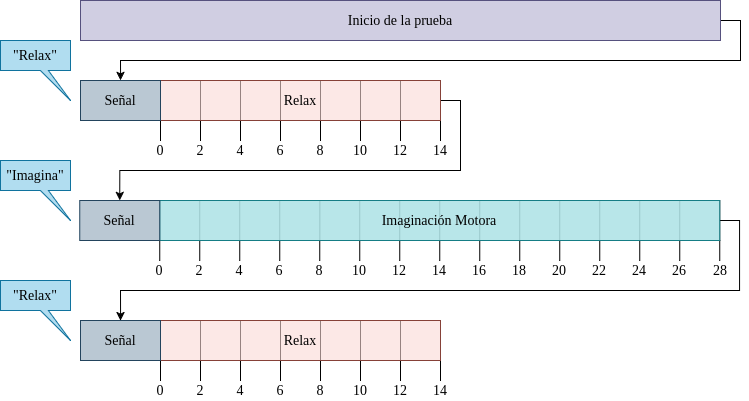
\includegraphics[width=1\textwidth]{img/ventanas.png}
    \caption{Estructura temporal de las ventanas EEG utilizadas durante cada ensayo. Adaptado de \cite{ferrero_BCIBased2021}.}
    \label{fig:ventanas}
\end{figure}


\subsubsection{Estructura y cuantificación del dataset}
A partir del protocolo experimental descrito, el dataset queda organizado jerárquicamente en sujetos, días, ensayos y ventanas temporales. En concreto, se dispone de:

\begin{itemize}
    \item 5 sujetos,
    \item 5 días consecutivos de adquisición por sujeto,
    \item 11 ensayos por día,
    \item 56 ventanas temporales por ensayo.
\end{itemize}

Por tanto, el número total de ventanas disponibles es:

\[
    5 \times 5 \times 11 \times 56 = 15400 \text{ ventanas}
\]

Cada ventana contiene \(27\) canales EEG y \(400\) muestras temporales. Así, los datos de entrada presentan inicialmente una estructura de tipo:

\[
    (15400, 27, 400)
\]

mientras que las etiquetas asociadas presentan una dimensión:

\[
    (15400, 1)
\]

donde cada etiqueta indica la clase correspondiente a la ventana temporal analizada.

Los datos originales se encuentran distribuidos en cuatro ficheros MATLAB diferenciados según la tarea experimental:

\begin{center}
    \begin{tabular}{|c|c|c|}
        \hline
                        & \textbf{Labels}                   & \textbf{Training}                   \\ \hline
        \textbf{Static} & \texttt{labels\_static\_data.mat} & \texttt{training\_static\_data.mat} \\ \hline
        \textbf{Motion} & \texttt{labels\_motion\_data.mat} & \texttt{training\_motion\_data.mat} \\ \hline
    \end{tabular}
\end{center}

Los ficheros de etiquetas contienen la intención de movimiento asociada a cada ventana temporal, mientras que los ficheros de entrenamiento almacenan las señales EEG correspondientes.

Con el objetivo de facilitar el entrenamiento y evaluación de los modelos propuestos, los datos fueron reorganizados en tensores que preservan la jerarquía original del dataset. La figura \ref{fig:tensor_input} muestra la estructura de los tensores de entrada y etiquetas obtenidos a partir de los datos originales.

\begin{figure}[H]
    \centering
    \fbox{
        \begin{minipage}{0.95\textwidth}
            \centering

            \textbf{Input tensor shape:} \((5, 5, 11, 56, 27, 400)\)

            \vspace{0.3cm}

            \begin{tabular}{c | c c c c c c}
                \textbf{Dim.} & 1     & 2    & 3      & 4       & 5        & 6       \\
                \textbf{Name} & Users & Days & Trials & Windows & Channels & Samples \\
                \textbf{Size} & 5     & 5    & 11     & 56      & 27       & 400
            \end{tabular}

            \vspace{0.6cm}

            \textbf{Labels tensor shape:} \((5, 5, 11, 56, 1)\)

            \vspace{0.3cm}

            \begin{tabular}{c | c c c c c}
                \textbf{Dim.} & 1     & 2    & 3      & 4       & 5     \\
                \textbf{Name} & Users & Days & Trials & Windows & Label \\
                \textbf{Size} & 5     & 5    & 11     & 56      & 1
            \end{tabular}

        \end{minipage}
    }
    \caption{Estructura jerárquica de los tensores de entrada y etiquetas utilizados en el modelo.}
    \label{fig:tensor_input}
\end{figure}


Esta organización permite mantener explícitamente la procedencia experimental de cada ventana, diferenciando el sujeto, el día, el ensayo y la posición temporal dentro del ensayo. Esto resulta especialmente útil para definir posteriormente las distintas estrategias de entrenamiento y evaluación empleadas en este trabajo.


\subsubsection{Preprocesamiento}


Previo al entrenamiento de los modelos, las señales EEG fueron sometidas a una etapa de preprocesamiento con el objetivo de reducir el ruido y conservar únicamente los componentes frecuenciales relevantes para las tareas mentales objetivo.

Se aplicaron dos filtros en la etapa inicial de preprocesamiento: un filtro notch a 50 Hz para reducir el ruido provocado por la red eléctrica y un filtro paso alto a 0.1 Hz para eliminar la componente continua y derivas lentas de la señal \cite{ferrero_BMIBased2021}. Se aplicó también el algoritmo H\(_\infty\) para la eliminación de artefactos oculares, que permite reducir la influencia de movimientos oculares y parpadeos en la señal EEG \cite{kilicarslan_RobustAdaptive2016}.

Finalmente, a cada canal EEG se le aplicó un filtro paso banda entre 8 y 40 Hz. Este rango frecuencial incluye principalmente las bandas \(\mu\) (8--13 Hz) y \(\beta\) (13--30 Hz), ampliamente utilizadas en aplicaciones \acrshort{bci} basadas en imaginación motora debido a su relación con la actividad cortical motora \cite{mirnaziri_UsingCombination2013}.

Posteriormente, se eliminaron los periodos correspondientes a instrucciones y segmentos iniciales no pertenecientes a las tareas mentales objetivo. De esta forma, el análisis se centró únicamente en las ventanas asociadas a relajación e imaginación motora.



    {\color{red}
        la Pipeline
        qué hace tu sistema de principio a fin

        Ejemplo:

        entrada: EEG

        procesamiento

        modelo

        salida: predicción


    }
